% !Mode:: "TeX:UTF-8"%確保文檔utf-8編碼
%新加入的命令如下: reduline showendnotes 
%新加入的环境如下:solution solutionorbox solutionorlines solutionordottedlines

\documentclass[12pt,twoside]{exam}
\newlength{\textpt}
\setlength{\textpt}{12pt}

\usepackage{teachingplan}
\usetikzlibrary{patterns,calc}

%写上答案或者不写上答案%
%\printanswers  


%讲知识点然后测试,测试通过继续下一个知识点。不通过给予小提示,然后继续测试,如果通过那么通过,如果还是不会做,那么继续讲解知识点,并讲解这个题目,然后重新给出一个题目重新测试。

%如果有精力,后面再准备一套中考真题。

%\excludecomment{knowledge}
\includecomment{knowledge}
%\excludecomment{Aquestions}
\includecomment{Aquestions}

\CenterWallPaper{1}{教案模板-2.pdf}

\newcommand{\keti}{力和运动}
\newcommand{\zhongdian}{1.力 2.弹力 3.重力 4.摩擦力 \\5.牛顿第一定律 6.力和运动 7.力的作图}
\firstpageheader{}{}{\today}
\begin{document}
\ThisCenterWallPaper{1}{教案模板-1.pdf}
\vspace*{80pt}
\keti \par
\zhongdian \par
\begin{knowledge}
\begin{flushright}
\begin{notecard}{12em}
\ttfamily
一切智慧皆来自你的内心。
\end{notecard}
\end{flushright}
\section{什么是力}
问同学,力是什么?

力最直观的感受手掌感受到了压力,这是我们人最直观的感受。但是就好比你摸到一个东西好烫高喊到:“啊,这东西温度好高啊。”一样,你不能把这种感觉作为温度的定义。

\subsection{力是物体对物体的作用}
关于力的定义初中物理书是这样说的:力是\uwave{物体对物体的作用}。

这句话很有深意,简单的理解就是力不能单独存在,如果某个物体受到了力,那么一定是有另外一个物体对它施加了某种作用。这个定义算不上某个公理,只是大家似乎潜移默化的都接受了。而且这句话还暗含这种思维:那就是标记了物体的起源。(我是这么理解这句话的,它属于人触觉压力感知模式的扩展,就好比你就是那个物体,然后你感受到了压力,那么就等同于你摸到另外那个物体了。)


\subsection{牛顿关于力的定义}
\subsubsection{伽利略之前}
在伽利略之前,人们比如说亚里士多德就认为力是物体保持运动状态的原因。可能那个时候也没有太多光滑的东西,然后你如果在粗糙的地面上推箱子,确实好像要不断施加力才能维持箱子的运动。

\subsubsection{伽利略的小车实验}
伽利略用实验的和数学的方式设计了大家熟知的斜面小车实验,通过实验他发现平面越光滑,小车受到的阻力越小,滑行的越远。于是他推断如果平面绝对的光滑,那么小车受到的阻力为零,它的速度就不会减慢,这样小车就会以恒定不变的速度永远运动下去。这样就推翻了亚里士多德关于力的定义的学说。

\begin{fig}{2012陕西30-1}
\end{fig}

\textbf{(2012陕西,30(1),2分)}图是牛顿第一定律的实验基础之一。让同一小车从斜面相同高度静止下滑,比较小车在不同水平面上通过的\answer[7em]{距离(路程)},据此可以推理得出:当水平面绝对光滑时,小车将做\answer[7em]{匀速直线运动}。

\textbf{(2013河北,15,2分)}第一位提出“物体的运动并不需要力来维持”的物理学家是(\answerline*[A])

\begin{oneparchoices}
\choice 伽利略
\choice 奥斯特
\choice 帕斯卡
\choice 阿基米德
\end{oneparchoices}

\subsubsection{牛顿第一定律}
牛顿在总结前人的成果和构建自己的力学体系时明确提出了牛顿第一定律:一切物体在没有受到力的作用的时,总保持\answerline*[静止]状态或\answer[7em]{匀速直线运动}状态。

这样反过来牛顿关于力的理解就是:如果某个物体运动状态发生了变化,那么我们就说这个物体受到了力。用初中物理的话语来说就是力可以改变物体的运动状态,还可以改变物体的形状(发生形变实际上物体部分运动状态发生了变化)。

由这个运动状态的变化(也就是速度的变化率——加速度)和力的关系就是著名的牛顿第二定律,这个高中才讨论。而牛顿还发现:相互作用的两个物体之间的力是大小相等,方向相反的——这就是牛顿第三定律。第二第三定律初中都不做要求,只需要对力的相互作用有一个概念即可。

比如说\leftnote{板书}苹果受到地球的吸引而下落,这个时候苹果也对地球有一个吸引力;比如说书压在课桌上,书对课桌有一个压力,而课桌对书则有一个支持力;再比如说汽车在马路上行驶,是因为汽车对马路有压力,马路很粗糙然后产生了摩擦力。车轮基于这个摩擦力从而产生了一个向前的推力,而马路则受到了车轮的向后的推力。——如果马路是绝对光滑的,车子是无法前进的,生活中车子雪地打滑就是这个原因。

\textbf{(2010云南昆明,23,5分)}图为某同学“探究牛顿第一定律”的实验装置。实验中该同学先后三次将同一木块放在同一斜面上的同一高度,然后分别用不同的力推了一下木块,使其沿斜面向下运动,逐渐改变水平面的粗糙程度,观察木块运动的距离,从而得出力和运动的关系。
\begin{linefig}{2010云南昆明23}
\end{linefig}

(1)该同学在实验操作中有一处明显的错误是(不要求解释错误的原因):\answer[20em]{分别用不同的力推了一下木块}。

(2)更正错误后进行实验,从实验中可观察到,随着摩擦力的逐渐减小,木块在水平面上运动的距离逐渐\answerline*[变长],运动的时间越来越\answerline*[长]。但由于实验中摩擦力\answer[7em]{不可能为零},所以不可能观察到木块在水平面上做匀速运动的情形。

(3)在上述实验观察分析的基础上,可以推测:如果摩擦力减小为零,水平面足够长,那么木块在水平面上的运动速度既不减小,也不增大,运动方向也不发生改变,木块将做\answer[8em]{匀速直线运动}。

\subsubsection{力的定义}
初中物理关于力的定义只是一种触觉感知模式的延伸,牛顿关于力的定义并没有触及力的本质,只是基于物体的运动来间接推断该物体可能受到了力,也许将来人们统一了各种各样的力之后会对力的本质有更深刻的理解吧。


\subsection{惯性}
一切物体都有保持原有运动状态(也就是牛顿第一定律描述的物体在不受力的情况下,总保持静止或匀速直线运动)的特性,我们把这种特性叫做\textbf{惯性}。牛顿第一定律也叫惯性定律。

举一些例子:比如车子开动,人向后倾(保持静止);车子向左拐弯,人向右倾(人保持原来运动方向不变);车子匀速行驶,人竖直向上跳起来,仍落回原地(人相对车子水平运动方向保持静止);车子突然停住,人向前冲(人保持向前运动)等等。

惯性的大小可以用物体所含的\textbf{质量}来衡量,质量越大,惯性就越大,质量不变则惯性不变。

\textbf{(2012河北,20,2分)}下列有关惯性的说法\dotuline{不正确}的是(\answerline*[B])
\begin{choices}
\choice 运动员跳远时助跑,利用了惯性。
\choice 司机驾车时系安全带,可以减小惯性。
\choice 自行车停止蹬踏后,仍继续前行,是因为人和车都具有惯性。
\choice 地球由西向东转,人竖直向上跳起来,仍落回原地,是因为人具有惯性。
\end{choices}

\textbf{(2012上海,11,3分)}地铁是上海市民的重要交通工具之一,当某列车启动时,该车的惯性不\answerline*[不变](选填“增大”、“不变”、“减小”),以站台为参照物,坐在车内的乘客是\answerline*[运动]的(选填“运动”或“静止”);列车驶过后,铁轨的温度会升高,这是通过\answerline*[做功]的方式改变其内能。\leftnote{第三问可忽略}


\section{力的作图}
\subsection{力的三要素}
力的三要素是力的\answerline*[大小],\answerline*[方向],\answerline*[作用点]。只要有一个要素发生变化,力的作用效果就会改变。

力的图示就是用一根带箭头的线段把力的三要素都表示出来。具体画的过程如下\leftnote{随便举个例子说明一下}:
\begin{enumerate}
\item 先画点,点表示力的作用点,这个点一般画在物体的重心上。
\item 再画线和箭头,线段的长度大致说明力的大小(主要是要表示清楚\uwave{线段长的力大}),箭头表示力的方向。
\item 最后旁边具体标上力的大小是多少牛顿,如果不知道可以不写。
\end{enumerate}


\textbf{(2012上海,17,3分)}重为4牛的球体静止在水平地面上,用力的图示法在图中画出它受到的重力$G$。
\begin{multicols}{2}
\begin{linefig}[0.8]{2012上海17-1}
\end{linefig}
\columnbreak
\begin{solution}
\begin{linefig}[0.9]{2012上海17-2}
\end{linefig}
\end{solution}
\end{multicols}

(2012河南,17,2分)如图所示,将一个小球放在竖直放置的弹簧上,用手向下压小球,松手后,小球在弹簧弹力作用下向上加速运动,不考虑空气阻力,请画出此时小球的的受力示意图。

\begin{linefig}[0.4]{2012河南17-1}
\end{linefig}


\section{二力平衡}
\subsection{力的合成基础}
实际上很难说出一个物体具体受了多少个力,但我们可以确定一个物体运动状态发生了改变,一定受到了力。它实际上可能受到好几个力,比如就以最简单的重力来说。一个物体受地球的吸引,要注意地球是由很多很多岩石组成的哦,也就是那个物体受到的重力实际上是受很多很多岩石的万有引力的吸引力的合力。合力作用在该物体上的效果和很多很多力作用在那个物体上的效果是完全或近似相同的(比如这些力还有一个附加于观察物的拉扯效果,如果大的话可能会把观察物拉碎。),于是我们在分析上方便起见就可以只研究那个合力(这在高中有专门的力的合成的讨论)。

初中物理有关力的合成我们需要掌握的有:
\begin{itemize}
\item 如果两个力方向完全相同,那么将合成一股力,这股力的方向和之前两个力的方向一样,大小是他们两者之和。
\item 如果两个力方向反向,且在同一直线上,那么他们将合成一股力,这股力的方向和之前两个力中力较大的那个一致,大小是他们两者之差。
\end{itemize}

\subsection{二力平衡}
如果在力的合成中出现了合力为零时的情况,那么这个时候物体就如牛顿第一定律所描述的那样,是不受力的状态,将保持静止或匀速直线运动状态。我们称这几个力为平衡力。

在初中物理有关平衡力的讨论只考虑二力平衡的情况,也就是两个力大小\\ \answerline*[相等],方向\answerline*[相反],作用于同一条直线上,那么这两个力处于二力平衡状态了。

虽然初中物理不考察加速度,但是常常有题目会涉及到加速或者速度改变的情形,这里需要提醒的是速度发生变化,那么物体的运动状态也就发生了变化,那么物体一定是受到力的,那么物体就一定是不处于二力平衡状态。具体简单的观念应该有:汽车加速,则有额外的动力加入,所以推力大于摩擦力。汽车减速,则摩擦力大于汽车的推动力,所以速度慢慢减下来了。

\textbf{问题:}人乘坐电梯时,电梯匀速上升时候电梯对人的支持力等于500N,则电梯加速上升的时候电梯对人的支持力\answerline*[大于]500N,电梯匀速下降的时候电梯对人的支持\answerline*[等于]500N,电梯加速下降的时候电梯对人的支持力\answerline*[小于]500N。(以上选填“小于”、“大于”、“等于”)

\textbf{(2013江苏苏州,21,2分)}小强用10N的水平推力匀速推动放在水平地面的课桌,则课桌受到地面对它的摩擦力的大小是\answerline*[10]N;某同学将该课桌内的书包拿走后,把课桌沿原路用水平力推回的过程中,课桌受到地面对它的摩擦力\answerline*[小于](小于/等于/大于)10N。\leftnote{第二问要求摩擦力知识}


\section{弹力}
物体受力时发生形变,不受力时又恢复原来的形状的特性叫做弹性。物体变形后不能自动恢复原来形状的特性叫做塑性。物体由于发生弹性形变而产生的力叫弹力。物体的弹性有一定的限度,使用时不能超过它们的弹性限度,否则会损坏它们。


\subsubsection{弹簧测力计}
测量力的大小的工具叫做测力计。实验室常用的测力计是\answer[7em]{弹簧测力计}。

\vspace{45pt}
\noindent
\begin{minipage}{\textwidth}
\begin{minipage}[c][6cm][c]{0.75\textwidth}
弹簧测力计的原理是在弹性限度范围内,弹簧伸长量于受到的拉力成正比。\\[10pt]

使用弹簧测力计的注意事项:
\begin{enumerate}
\item[①] 检查指针是否在零刻度线处,没有调节之。
\item[②] 看量程,加载弹簧测力计上的力不能超过它的量程。
\item[③] 看分度值,认清一小格多少牛。力的单位是牛顿,字母表示是N。
\item[④] 沿轴线方向用力,别让弹簧指针卡住。读数时视线与刻度面垂直。
\end{enumerate}
\end{minipage}\hfill
\begin{minipage}[c][6cm][c]{0.25\textwidth}
\begin{linefig}[0.7]{弹簧测力计}
\end{linefig}
\end{minipage} 
\end{minipage} 

\vspace{50pt}
\textbf{(2013贵州贵阳,30,6分)}小帆在练习使用弹簧测力计(以下简称测力计)测物体重力时,她先将测力计竖直放置,反复几次轻拉挂钩后,测力计的指针位置如图甲所示。
\begin{linefig}[0.8]{2013贵州贵阳30}
\end{linefig}
(1)此测力计的量程是0~\answerline*[5]N。若此时她将一个3N重的物体悬挂于挂钩上,静止后,测力计的示数应\answerline*[大于]3N(选填“大于”、“等于”、“小于”)。

(2)在老师的指导下,小帆调整好了测力计,将某物体悬挂好,物体静止后,指针指在如图乙所示的位置,则次物体的重力$G$=\answerline*[2.6]N。

(3)老师强调:“只有当物体静止或匀速直线运动时才能读数。”请你解释其中的原因:\begin{solutionorlines}[4em]
只有物体静止时,重力和拉力才处于二力平衡状态,重力才等于拉力,弹簧所测拉力才能表示物体的重力。
\end{solutionorlines}

(4)小帆使测力计和物体加速上升的过程中,发现测力计的示数大于物体的实际重力。请解释示数变大的原因:
\begin{solutionorbox}[4em]
物体加速上升,物体不再受力平衡,弹簧所受的拉力大于物体的重力,导致示数变大。
\end{solutionorbox}


\section{重力}
宇宙间任何两个物体,都存在互相吸引的力,这就是万有引力。由于地球的吸引而使物体受到的力,叫做重力。地球上所有物体都受到重力的作用。重力的施力物体是地球。

通常物体所受重力的大小叫做该物体的重量。物体所受的重力跟它的质量成正比,它们之间的关系是$G=mg$。(单位?g=9.8N/kg,要求不是很严格的情况下,可视作10N/kg)

这里简单将一下质量,重量和重力的关系,以天平在月球上和太空中为例讲解。


\subsection{重心}
重力的方向总是\answerline*[竖直向下]的。应用:重垂线

重力在物体上的作用点叫做重心。形状规则的物体的重心在它的几何中心。

\textbf{(2012北京,11,2分)}图是描述地球上不同位置的人释放手中石块的四个示意图,图中虚线表示石块下落的路径,则对石块下落路径的描述最接近实际的示意图是(\answerline*[B])
\begin{linefig}{2012北京11}
\end{linefig}


\section{摩擦力}
两个互相接触的物体,当它们做相对运动时,在接触面上产生的阻碍(所以摩擦力的方向总是与运动方向相反)相对运动的力叫摩擦力。摩擦力的方向总是跟物体运动方向(或运动趋势方向)相反。

\leftnote{简单手绘}当你轻轻推一个箱子是,箱子不动,这个时候箱子的受力是推力\answerline*[等于]摩擦力(此时的摩擦力是\textbf{静摩擦力})。而当你再加把劲推动箱子时,箱子还是不动,这个时候还有推力等于摩擦力,而且此时的摩擦力是\answerline*[大于]之前轻轻推时箱子所受到的摩擦力的。当你再加把劲的时候箱子终于推动了,这个时候摩擦力变成了\textbf{滑动摩擦力}。

滑动摩擦力既跟作用在物体表面的压力有关,又跟接触面的粗糙程度有关。压力越大,则滑动摩擦力\answerline*[越大],接触面越粗糙,则滑动摩擦力\answerline*[越大]。

如果你把箱子推动了,此时物体所受到的滑动摩擦力是一定的,因为箱子的重量不变,则箱子对地压力不变,箱子和地面接触面的粗糙程度不变,所以滑动摩擦力的大小总是一定的,而不管这个箱子是加速运动啊还是减速运动还是匀速运动。其中如果箱子是匀速运动的,则我们有箱子所受到的推力\answerline*[等于]箱子所受到的摩擦力。

最后摩擦还有一种情形:\textbf{滚动摩擦},滚动摩擦比滑动摩擦\uwave{小得多}。比如说埃及人修金字塔运送石头的时候下面铺上滚木。

我们应增大有益摩擦,减小有害摩擦。\\
增大摩擦的方法:增加接触面的粗慥程度,增加压力,变滚动为滑动;\\
减小摩擦的方法:减小接触面的粗糙程度(使接触面光滑),减小压力,使两个互相接触的表面分开(气垫船,磁悬浮列车。),变滑动为滚动。

\textbf{(2011甘肃兰州,17,2分)}在水平桌面上有一质量为1kg的长方体。用4N的水平拉力向右拉,长方体静止不动,此时它所受的摩擦力为\answerline*[4]N;拉力增大至6N时长方体做匀速直线运动;若拉力增大至8N时长方体所受的摩擦力为\answerline*[6]N。




\section{总结}


\textbf{(2012江苏无锡,25,8分)}



\end{knowledge}





\begin{Aquestions}
\newpage
\section{题库A}
\begin{questions}
\question
\textbf{(2009广州,9,3分)}如图所示,将木块放在压缩了的弹簧旁,释放弹簧,木块沿水平地面向右运动,离开弹簧后,木块运动一段距离后停下来。下列说法正确的是(\answerline*[B])

\noindent
\begin{minipage}{\textwidth}
\begin{minipage}[c][6cm][c]{0.7\textwidth}
\begin{choices}
\choice 木块所受摩擦力使木块由静止开始运动
\choice 弹簧对木块的弹力使木块由静止开始运动
\choice 木块所受摩擦力不会改变木块的运动状态
\choice 木块最终停止运动是由于失去弹簧的弹力作用
\end{choices}
\end{minipage}\hfill
\begin{minipage}[c][6cm][c]{0.3\textwidth}
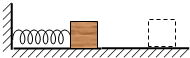
\includegraphics[scale=0.8]{figures/2009广州9.png} 
\end{minipage} 
\end{minipage} 


\end{questions}
\end{Aquestions}









%
\ThisCenterWallPaper{1}{教案模板-3.pdf}

\end{document}



